\documentclass[10pt, twocolumn, letterpaper]{article}

%% Language and font encodings
\usepackage[english]{babel}
\usepackage[utf8x]{inputenc}
\usepackage[T1]{fontenc}

%% Sets page size and margins
\usepackage[a4paper, top=3cm, bottom=2cm, left=3cm, right=3cm, marginparwidth=1.75cm]{geometry}

%% Useful packages
\usepackage{amsmath, graphicx, natbib, multicol}
\usepackage[colorinlistoftodos]{todonotes}
\usepackage[colorlinks=true, allcolors=blue]{hyperref}
\bibliographystyle{unsrt}
%% Title
\title{
		\usefont{OT1}{bch}{b}{n}
		\normalfont \normalsize \textsc{STEM Fellowship Big Data Challenge 2020} \\ [10pt]
		\huge Project Title \\
}
\selectlanguage{english}
\usepackage{authblk}
\author[1]{Eddie Guo}
\author[2]{Mehul Gupta}
\author[1]{Pouria Torabi}
\author[2]{Sunand Kannappan}
\affil[1]{University of Alberta}
\affil[2]{University of Calgary}


\begin{document}
\maketitle

% Abstract
\begin{abstract}
    Your abstract will get published whether or not your team wins the challenge, so make sure to do a good job! It should reflect the objectives, methodology and findings of the research project. When writing your abstract, choose the right (amount of) words to convey your information. Avoid long sentences and long-winded explanations as they could make the reader lose focus. The order of your writing is also important. Maintain a logical order to your writing so that the reader links each aspect of your work coherently. Introduction/Background: Explains what problem the study examined and why. You may provide some background to the project, and the motivation behind it. Materials and Methods: Describes the data sources used and methodologies adopted for the data analysis. Key Findings/Results: Outlines the discoveries/what was observed from the analysis. When describing your results, strive to focus on the main finding(s), and list no more than two or three points. Conclusion: Provide a general interpretation of the results, specifying what is new/innovative of your project, and give any important recommendation for future research.Once you've written these, delete the keywords, edit for flow, and you have your abstract.
\end{abstract} \vspace{1em}

% Keywords
\noindent {\textbf{Keywords}\\
pick, 3-5, good, keywords}


% Introduction
\section{Introduction}
Before we get to the actual introduction, welcome to Overleaf, as well as \LaTeX\ itself! Although \LaTeX\ certainly has its quirks, we hope that by contrasting the template you see here with the compiled document on the right side, you can get an intuitive sense of how to work with it. Anyhow, let's begin!

Another thing before the introduction; here, I'm going attach a citation to this sentence. Scroll on down to the bibliography section of the \LaTeX\ code if you'd like to see the other end of the built-in references system. The numbering is all handled in-house -- you just have to assign each reference a key, and Overleaf takes care of the rest!

On with the actual introduction. Here is where you'd introduce the context surrounding your study. What led you to the question you ended up asking? Why is it relevant? Which fields of science is your question based around?

You could also potentially discuss why Altmetrics themselves are relevant and were important in answering the question your team conceptualized, especially in comparison to using more traditional metrics such as citations.

While the structure of the previous parts of the introduction can be relatively variable, you must make sure to provide a brief overview of the study itself, and the methods you used to accomplish it. Obviously, excessive detail is not necessary (that's what the next section is for). Lastly, be sure to make mention of the potential implications of your findings, but once again remember that you'll be going into more detail about that in the discussion.

Also, please do remember that the STEM Fellowship Journal is an open access journal, which means that the full final papers of previous BDC winners are a simple Google search away!


% Materials and Methods
\section{Materials \& Methods}
This is where you talk about the methods used to carry out the study. Be as concise and to-the-point as possible, and remember - \textbf{do not justify your methods here!} You simply need to state what you did. You can (and probably should) mention the purpose of using a certain computational tool within the context of what you set out to achieve, but mentioning things like 'it's particularly efficient at this and better than all competing computational tools' is unnecessary in the methods section. However, you can definitely talk about all of this in the discussion, and talk about why your methods are, say, the most effective ones for the task.

Think of this section as a technical manual of sorts, that another team of researchers could read and easily follow in order to replicate what you did to carry out this study.

Because of the straightforward nature of the methods section, this might be the one your team wants to write first. It's essentially you just documenting what your team has already done, which should be no problem to write, since you will already have an established workflow by this point.

% Results
\section{Results}
The results section is probably next easiest to write after the Methods section, since it essentially boils down to presenting your data. If anything, the production of good, high quality figures is the most important and potentially time-consuming part of this. However, make sure to not analyze any of your results here! All of that belongs in the discussion.

Including figures into \LaTeX\ can seem intimidating at first, but Overleaf makes it easy: simply click the 'Project' button above, select 'Files', and upload away from your computer. Then, insert the file name into the appropriate section of the code below. Figure 1  shows the output of such code. A pretty good guide to formatting figures can be found at \url{https://en.wikibooks.org/wiki/LaTeX/Floats,_Figures_and_Captions#Figures}. \vspace{1em}

{\scriptsize
\begin{verbatim}
\begin{figure}
    \centering
    \includegraphics[width=0.4\textwidth]{test.png}
    \caption{Hello!}
\end{figure}
\end{verbatim}
}

\begin{figure}
  \centering
  \includegraphics[width=0.4\textwidth]{Figures/test.png}
  \caption{Notice how \LaTeX\ automatically numbers this figure.}
\end{figure}


% Discussion
\section{Discussion}
And here is the 'meat' of the paper, so to speak. This is where you interpret your results, pointing out interesting trends within your data and how they relate to your initial hypothesis. This is also the place to justify your methodology, if you're so inclined (i.e. Why did you specifically use a certain statistical test over another? Why this tool over that tool?). Lastly, you're going to want to discuss potential sources of error. Make sure to make explicit reference to Figures/tables when discussing your data; it can be helpful to walk the reader through your own personal interpretation of each figure in order. Although we recommend looking at past winning papers over at the STEM Fellowship Journal's website anyways, referring to those papers might prove most helpful when it comes to writing your discussion.


% Conclusions
\section*{Conclusions}
What are the long-term implications of your findings? Wrap up your discussion succinctly while pointing out the significance of your work as well as it what it means for the fields you examined as much as possible. Lastly, suggest ideas for future studies that could build on your work, and justify why they might be useful. Otherwise, you're all done!


% Acknowledgements
\section*{Acknowledgements}
Anyone to thank/credit for helping your team along the way? This is the place to do it!


\bibliography{bibliography}
\end{document}
